{
\chapter{The SoLid Experiment}
\section{Introduction}

\subsection{Detector Technology}
This has some potential draw backs: in cases where multiple $x$ fibres are in co-incidence with multiple $y$ fibres (e.g. in the case of an angled muon), it can be difficult to recover the cube information (but not impossible - see section: [todo add section]). As will be seen, these degenerate cases are rare (relative to the timing resolution of the detector) and is not a limiting factor for the majority of analyses at SM1.

\section{SM1 Prototype}
The SoLid Module 1 (SM1) detector is a prototype module of the full SoLid detector. Constructed and commissioned in January 2015, this detector aims to prove many of the design principles of the full detector, including the power of segmentation and appropriate handles of backgrounds. This section outlines the module technology (which differs slightly from that planned for SoLid) and event reconstruction, preparing the reader for SM1 results in the following chapter. 

\subsection{Detector design}
\subsubsection{Coordinate system}
The coordinate system at SM1 used in the following sections is shown in figure~\ref{fig:sm1_codn_system}.

\begin{figure}
\begin{center}
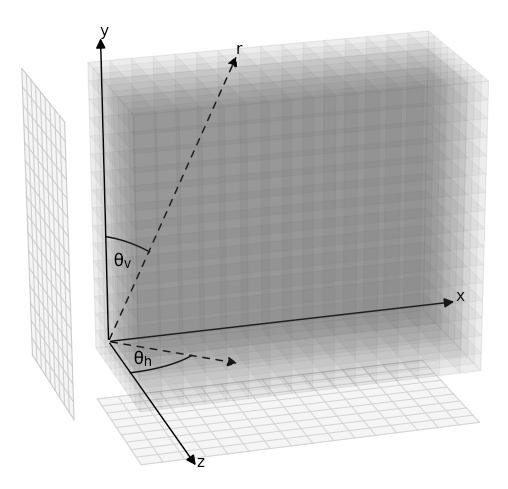
\includegraphics[width=1.0\columnwidth]{Chapters/solid1/codnSystem.png}
\caption{The coordinate system used for SM1. A right-handed system is used, where the y axis points vertically upwards, and the z axis points radially away from the reactor. The origin is in the center of the bottom left cube (as seen when looking towards the reactor) that is closest to the reactor and far left. For tracking purposes, it is useful to define the following two angles: $\theta_v$, the angle between some vector r and the y axis, and $\theta_h$, the angle between the z axis and the component of r in the xz plane. The two photo-detector arrays - $xz$ and $yz$ - are also visible.}
\label{fig:sm1_codn_system}
\end{center}
\end{figure}

\subsubsection{Detector configuration}
The detector technology used at SM1 is identical to that planned for the full SoLid detector, however there are some configuration differences, many of which are consequences of the analyses of SM1 data. There are the following similarities and differences:

\begin{itemize} 
\item \textbf{Cubes} The module is composed of $9$ planes of cubes. Each plane is square, with $16$ cubes along each side. This gives a total of $2304$ cubes, and a mass of $294kg$ ($~10\%$ of the full planned mass). As above, each cube is made of Polyvinyl toluene (PVT), and light shielding is achieved by wrapping each cube in Tyvek.

\item \textbf{Light fibres} Each row and column of cubes in a plane contains a single wavelength shifting fibre (in contrast to SoLid, which will have two fibres per row and column for increased light yield). Each fibre is attached to a silicon photomultiplier. No information is  shared between planes at SM1 during the detector trigger or readout (again, in contrast to SoLid, where the trigger is planned to be shared across planes). 

\item \textbf{Silicon photomultipliers and readout} Each light fibre is read out using a silicon photomultiplier. The DAQ readout uses a $62.5MHz$ clock, which allows for $16ns$ precision in the sampling of the waveforms. [todo: a note on the precision of the waveforms bin units]

\item \textbf{Muon Vetos} Each light fibre is read out using a silicon photomultiplier. The DAQ readout uses a $62.5MHz$ clock, which allows for $16ns$ precision in the sampling of the waveforms. [todo: a note on the precision of the waveforms bin units]
\end{itemize}

\subsection{Triggers and data format}
SM1 has two kinds of triggers:
\begin{itemize}
\item \textbf{Random trigger mode} All channels are periodically read out simultaneously. The default rate is $0.2Hz$ and waveforms are $256$ bins in length.
\item \textbf{XY Co-incidence trigger} To trigger, at least one X channel and one Y channel in the same plane must be above a pre-set threshold within a time window. At this point, all channels above threshold and in co-incidence in that plane are read out. The default time window is $48ns$, with a default threshold of $170ADC$. These values have been optimised to maximise the data output of SM1, which is [todo: get max data rate].
\end{itemize}

$\newline$
The motivation for a coincidence trigger is related to the dark rate of the SiPMs. [todo purity estimate, use real data?].

$\newline$
In both trigger modes, waveforms of length $256$ bins are written to disk with $16$ bit integers precision - there is no processing of these waveforms in hardware. This format is chosen to increase understanding of the event signatures outlined above - in particular, for neutron identification. Since SoLid will have a separate trigger for neutrons, studies with SM1 waveforms are invaluable to optimise the neutron identification efficiency and purity.

\subsection{Event reconstruction}
The event reconstruction at SM1 composes of several data processing stages. Typically, each stage of reconstruction involves some form of pattern recognition (e.g. looking for co-incident signals, or the application of cuts), and often resulting in a reduced data format. Below are brief descriptions of the different stages of event reconstruction, used to identify the three different SoLid signatures outlined above:

\begin{itemize}
\item \textbf{Peak finding}
Since waveforms may contain multiple peaks (particularly in the case of random trigger mode), a peak finding algorithm is used to locate signals that pass above some threshold. This step is used for both kinds of signals - neutron and electromagnetic - for seeding later stages of the analysis, such as neutron ID or EM peak fitting.

\item \textbf{Clustering}
A clustering step is used to identify coincident channels touching eachother on either the xz or yz planes (for further details on the clustering algorithm, see section: [todo velo clustering section]). This step is used mainly for muon identification, since the most likely cause of large clusters in the passing of a muon. In the case of cube events, these are classed as single hit clusters and used later during cube resolving algorithms. 

\item \textbf{Tracking}
This step of reconstruction is exclusive for tracks and their pattern recognition - single cube events are not considered. As stated above, the signature of tracks are at least one large cluster on a detector arrary, with relatively high peak amplitudes. Given the expected angular distribution of cosmic tracks suggests vertical tracks will dominate, it is sufficient to search for large clusters on the $yz$ detector array (i.e. clusters formed of horizontal fibres) that are in coincidence with any size cluster on the $xz$ detector array. 

\item \textbf{Track fit}
Similar to section [todo: add velo tracking reference], tracks found in SM1 are parametrised as straight lints by four parameters as a function of $z$ position:

\begin{itemize}
\item $c_x$ and $c_y$, $x$ and $y$ positions of the track at $z=0$. 
\item $m_x$ and $m_y$, gradients along $x$ and $y$ with respect to the $z$ axis (gradients are assumed to be constant for the track whilst passing through SM1 [todo: some estimate of muon scattering]). 
\end{itemize}

Using these parameters, the $x$ and $y$ positions of tracks as a function of $z$ can be found using the following expressions:

\begin{itemize}
\item $x(z) = m_x \cdot z + c_x$
\item $y(z) = m_y \cdot z + c_y$
\end{itemize}

\item \textbf{Cube resolving and neutron identification}
Events resulting in the scintillation of a single cube are found by a similar process to that of the tracking, with the cluster size cuts limited to just size one clusters. Neutron identification methods can now be applied to the waveforms forming this cube and using the peak seed position. 

\end{itemize}

\section{Tracking performance}
This section focuses on the understanding of the tracks found at SM1 and the tracking performance, including the distributions of track parameters found at SM1, efficiency calculations and purity estimates. This is to prepare the reader for many of the discussions that follow in the next chapter, where these tracks are used for calibration and resolution studies. As will be seen, given tracks are abundant at SM1 [todo: add simple over-the-top-estimate], less emphasis is given to tracking efficiency, in favour of using simpler algorithms, whose limits and features can be better understood.

$\newline$ 
As outlined above, there are two parameters used in the track reconstruction: minimum cluster size on the $yz$ detector array, and a time coincidence window. To best understand the influence of the former cut and the overall efficiency, a toy monte carlo data set is generated according to pre-defined track parameter distributions, with the detector segmentation effects applied. This data set is then used to test the clustering and tracking algorithm efficiencies (note: the aim is not to create a simulation that describes all effects of SM1 - rather to test effects of segmentation on reconstruction algorithms and understand their associated efficiencies). 

\subsection{Path length resolution}
An important quantity used in the next chapter is the path length of a track through a particular cube (or set of cubes). To measure what effect segmentation has on such calculations, consider the path length through a plane of SM1 cubes. Given the above parametrisation of the muon track, the path length through a plane $\Delta r$ is given as:

\begin{center}
\begin{eqnarray} 
( \Delta r) ^2 &=& ( \Delta x )^2 + ( \Delta y )^2 + ( \Delta z )^2 \nonumber \\
&=& ( \Delta x )^2 + ( \Delta y )^2 + r_{Cube}^2 \nonumber \\
&=& (m_x^2 + m_y^2 + 1) \cdot r_{cube}^2 \nonumber \\
\end{eqnarray}
\end{center}

where $r_{Cube}$ is the length of a cube side. By comparing the values of $m_x$ and $m_y$ from simulation with those of the reconstructed tracks, the path length calculation can be optimised. An example residual distribution of this quantity is shown in figre~\ref{fig:pathlengthResiduals}. Similarly to section [todo: ref velo residuals], the width of a Gaussian fit to this residual is taken as the resolution (note: the tails of this distribution are discussed later). Two strategies are used for optimising the path length resolution:

\begin{figure}
\begin{center}
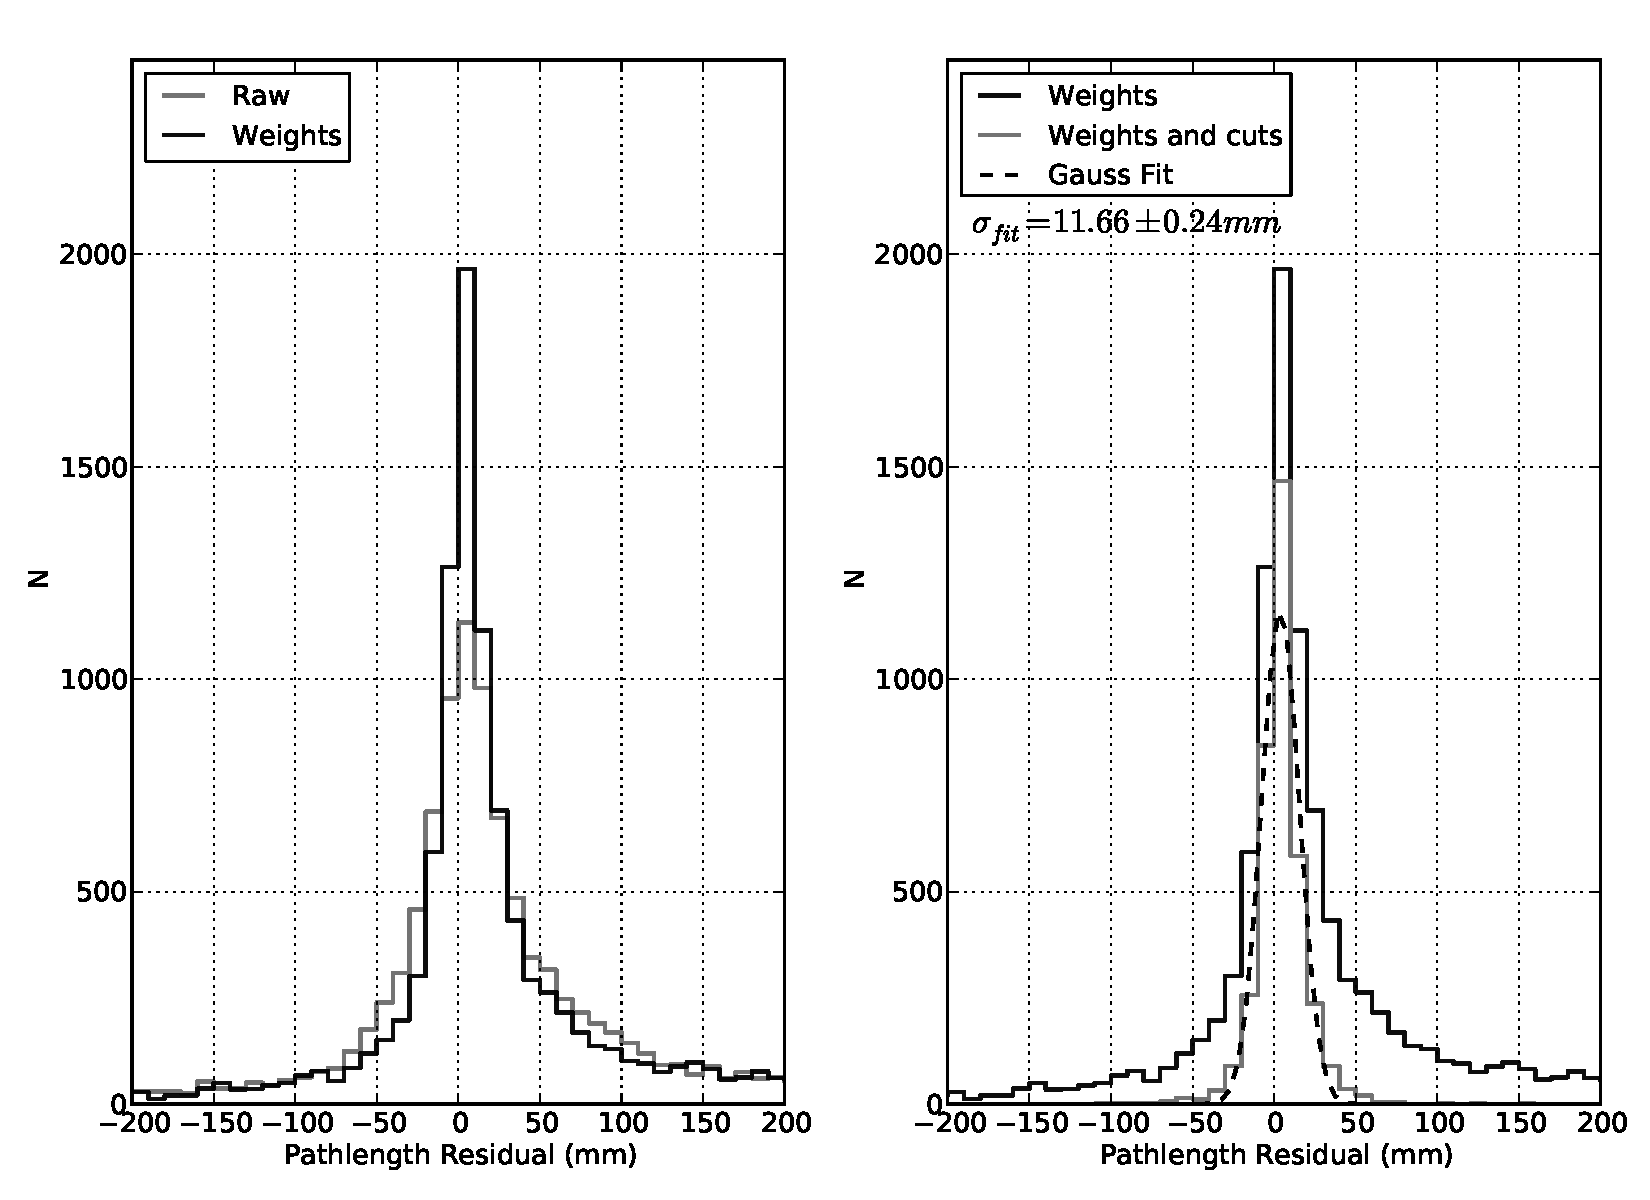
\includegraphics[width=1.0\columnwidth]{Chapters/solid1/pathlengthComparisons.pdf}
\caption{Path length residuals for simulated tracks passing through SM1, for various applied optimisation. Left: comparison between non-optimised (raw) residuals with weighted track fit. Right: comparison between weighted track fit and quality cuts.}
\label{fig:sm1_codn_system}
\end{center}
\end{figure}


\begin{itemize}
\item \textbf{Energy weighting} The linear regression used during the track fit assumed each data point is weighted equally. This is intuitively inaccurate, since the actual path-length through a row of cubes varies significantly. Since the energy measurements from each fibre give a measure of the time spent in that row of cubes, energy can be used as a weight in the track fit. Consider weighting each data point in the track fit by the following quantity:

\begin{center}
\begin{equation}
w = energy^alpha
\end{equation}
\end{center}

where alpha is some quantity that can be optimised by simulation [todo: reference velo cluster fit section]. By scanning over a range of $\alpha$, an optimum value of $\alpha = 1.5$ is found (figure~\ref{fig:trackWeightScan}, and the benefits of this weighting are shown in figure~\ref{fig:pathlengthResiduals} and table [todo: table]. 

\begin{figure}
\begin{center}
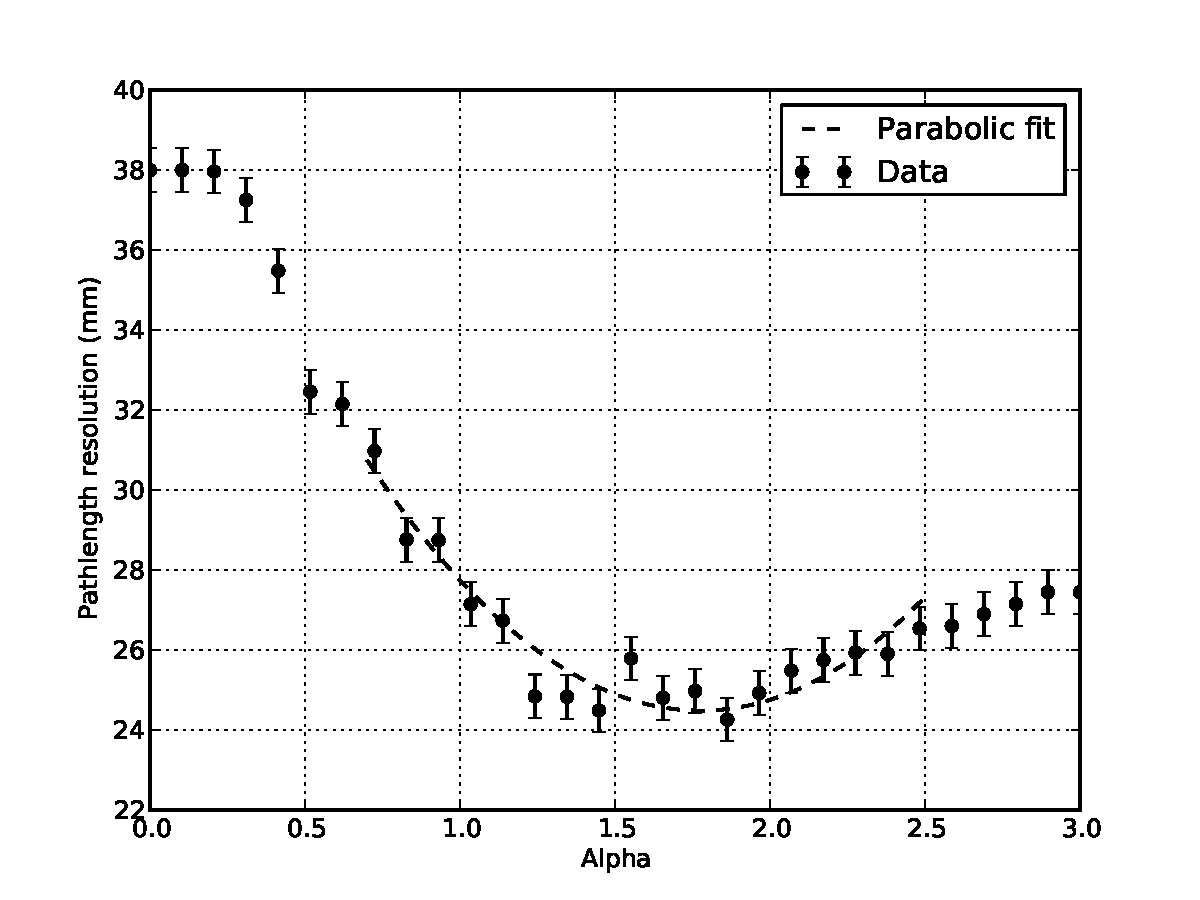
\includegraphics[width=0.75\columnwidth]{Chapters/solid1/alphaResScan.pdf}
\caption{}
\label{fig:trackWeightScan}
\end{center}
\end{figure}

\item \textbf{Quality cuts} 
Cuts on track parameters can be used to exclude sets of tracks that are known to have large errors in their reconstruction. For example, tracks that intercept a small number of fibres (e.g. clipping the corner of SM1) rely on fewer points in the track fit, which may lead to increased errors. This technique results in fewer tracks available for following studies, therefore there is a balance between statistics and resolution.

$\newline$
Two cuts in particular are explored: 
\begin{itemize}
\item \textbf{Minimum cluster size cut} - applied to both detector arrays ($xz$ and $yz$). This cut ensures tracks pass through enough fibres to reconstruct the track accuratly.

\item \textbf{Maximum pathlength cut} - tracks with a high pathlength through a detector are the main contribution to the tails of the pathlength residual. 

\end{itemize}

$\newline$
Scans over these two cuts are shown in figure~\ref{fig:pathlengthCutScans}. An optimal value to balance the loss of statistics with accuracy is chosen it be:

\begin{figure}
\begin{center}
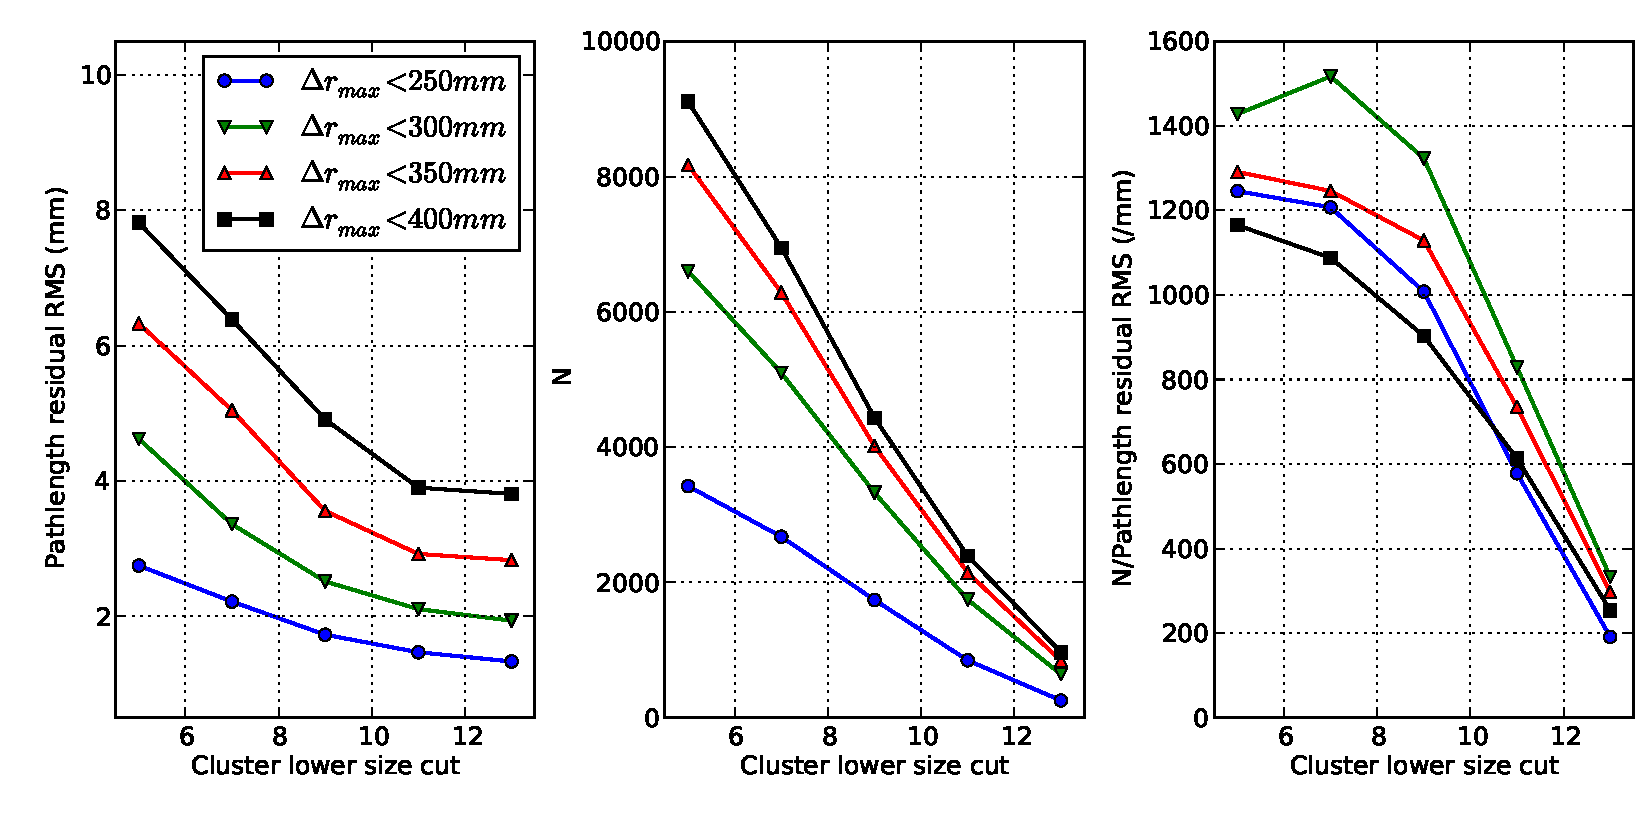
\includegraphics[width=1.0\columnwidth]{Chapters/solid1/pathlengthCutScans.pdf}
\caption{}
\label{fig:pathlengthCutScans}
\end{center}
\end{figure}

$\newline$
\begin{center}
$\Delta r < 300mm$, Minimum cluster size $>= 7$
\end{center}

\end{itemize}
}